\documentclass{standalone}
\usepackage{tikz}
\makeatletter\AtBeginDocument{\@buildstepset{1,2,3,4,5,6}}\makeatother
\usetikzlibrary{intersections, calc}
\usepackage{hsbcommon}
    \begin{document}
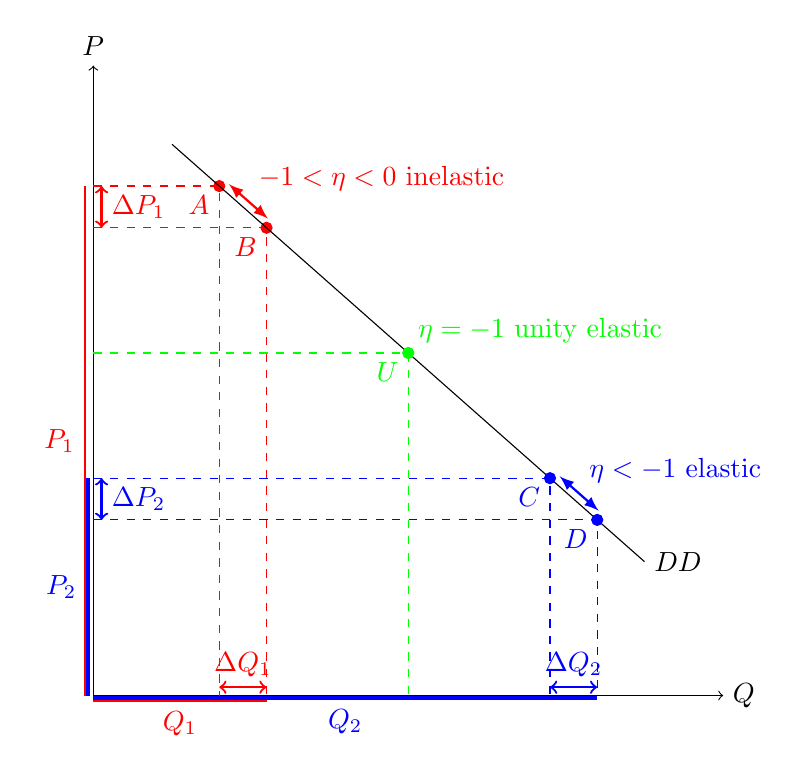
\begin{tikzpicture}
        \draw[->] (0,0) node[below] {\phantom{$X_i$}} -- (8,0) node[right] (Q) {$Q$};
        \draw[->] (0,0) node[left] {\phantom{$Y_mi$}} -- (0,8) node[above] (P) {$P$};

        \coordinate (A) at (1,7);
        \coordinate (F) at (7,1.7);
        % \coordinate (B) at ($(A)!0.1!(F)$);
        \coordinate (C) at ($(A)!0.1!(F)$);;
        \coordinate (D) at ($(A)!0.2!(F)$);
        
        \coordinate (D2) at ($(A)!0.8!(F)$);
        \coordinate (E) at ($(A)!0.9!(F)$);

 

        \ifstep{1}{
\begin{scope}[color=red]

            \filldraw (C) circle (2pt) node[below left] {$A$};
            \filldraw (D) circle (2pt) node[below left] {$B$};

            \draw[dashed]  (0, |- C) -- (C) -- (C |-,0);
            \draw[dashed]  (0, |- D) -- (D) -- (D |-,0);

            \draw[thick, <->,xshift=3pt] (0, |- C)  -- node [right] {$\Delta P_1$} (0, |- D);
            \draw[thick] ([xshift=-3pt]0, |- C) -- node[left] {$P_1$} ([xshift=-3pt]0,0);
            
            \draw[thick, <->,yshift=3pt] (C |-,0) -- node [above] {$\Delta Q_1$} (D |-,0) ;
            \draw[thick] ([yshift=-2pt]0,0) -- node[below] {$Q_1$} ([yshift=-2pt]D |-,0);

            \draw[thick, shorten >=2pt, ,shorten <=2pt,<->, >=latex,] ([xshift=2pt,yshift=2pt]C) -- node [above right] {$-1 < \eta<0$ inelastic} ([xshift=2pt,yshift=2pt]D);
            
        \end{scope}
}

        
        \draw [name path=demand] plot  coordinates {(A)  (F)};
        \node[right] at (F) {$DD$};

        % \node at (5,8) {\parbox{20ex}{between $A$ and $B$: inelastic demand}};
        
        \ifstep{2}{
\begin{scope}[color=blue]

            \filldraw (E) circle (2pt) node[below left] {$D$};
            \filldraw (D2) circle (2pt) node[below left] {$C$};            

            \draw[dashed]  (0, |- D2)  --  (D2) --  (D2 |-,0);
            \draw[dashed]  (0, |- E) -- (E) -- (E |-,0);
            
            \draw[thick, <->,xshift=3pt] (0, |- D2) -- node [right] {$\Delta P_2$} (0, |- E);
            \draw[ultra thick] ([xshift=-2pt]0, |- D2) -- node[left] {$P_2$}  ([xshift=-2pt]0,0);
            \draw[thick, <->,yshift=3pt] (D2 |-,0) -- node [above] {$\Delta Q_2$} (E |-,0);
            
            \draw[thick,shorten >=2pt, shorten <=2pt, <->, >=latex] ([xshift=2pt,yshift=2pt] D2) -- node [above right] {$\eta<-1$ elastic} ([xshift=2pt,yshift=2pt] E);
            \draw[ultra thick] ([yshift=-1pt]0,0) -- node[below] {$Q_2$} ([yshift=-1pt]E |-,0);

            
        \end{scope}
}

        \ifstep{3}{
\begin{scope}[color=green]

            \coordinate (G) at ($(A)!0.5!(F)$);
            \filldraw (G) node[below left] {$U$} circle (2pt);
            \node[above right] at (G) {$\eta=-1$ unity elastic};
            \draw[dashed] (0,|- G) -- (G) -- (G |-,0);
        \end{scope}
}

 
        
    \end{tikzpicture}
\end{document}
